\documentclass[a4paper, 12pt]{article}
\usepackage[a4paper, total={6in, 10in}]{geometry}
\usepackage{cmap}
\usepackage[T2A]{fontenc}
\usepackage[utf8]{inputenc}
\usepackage[russian, english]{babel}
\usepackage{statmath}
\usepackage{amsmath}
\usepackage{graphicx}
\usepackage{amssymb}
\usepackage{color}
\usepackage{hyperref}
\hypersetup{
    colorlinks=true,
    linktoc=all,
    linkcolor=black,
    urlcolor=black}
    
\setlength{\parindent}{0pt}

\begin{document}
\tableofcontents
\pagebreak

\part{Модуль 3}

\section{Гетероскедастичность}

\begin{itemize}
    \item Оценки несмещенные
    \item Несостоятельные
    \item Неэффективные
    \item ТГМ не выполняется $\rightarrow$ МНК-оценки не являются BLUE
    \item Гипотезы не работают
\end{itemize}

\subsection{Тест Голдфелда-Квандта}

\[\begin{cases}
    H_{0}: \textrm{Гомоскедастичность } (\sigma_{i}^{2} = \sigma_{\varepsilon}^{2}) \\
    H_{1}: \textrm{Гетероскедастичность } (\sigma_{i} \sim X_{ji} для нек. X_{j})
\end{cases}\]

\begin{enumerate}
    \item Упорядочить наблюдения
    \item Разделить наблюдения на 3 части
    \item Отдельно оценить регрессии и сохранить RSS
    \item $F(n_{2} - k, n_{1} - k) = \frac{RSS_{2}/(n_{2} - k)}{RSS_{1} / (n_{1} - k)}$
\end{enumerate}

\subsection{Тест Глейзера}

\[\begin{cases}
    H_{0}: \sigma_{i}^{2} = \sigma_{u}^{2} \\
    H_{1}: \sigma_{i} \sim X^{\gamma}, \gamma = \{\gamma = 1, \gamma = 1/2, \gamma = -1\}
\end{cases}\]

\begin{enumerate}
    \item Сохраняются остатки
    \item Если $\beta$ значима хотя бы для одной из регрессий, то имеем гетероскедастичность:
    \begin{enumerate}
        \item $|e_{i}| = \alpha + \beta X_{i} + u_{i}$
        \item $|e_{i}| = \alpha + \beta \sqrt{X_{i}} + u_{i}$
        \item $|e_{i}| = \alpha + \beta \frac{1}{X_{i}} + u_{i}$
    \end{enumerate}
\end{enumerate}

\subsection{Тест Уайта}

\[\begin{cases}
    H_{0}: \textrm{Гомоскедастичность} \\
    H_{1}: \textrm{Гетероскедастичность}
\end{cases}\]

\begin{center}
    \textit{Вид гетероскедастичности не специфицируется}
\end{center}

\begin{enumerate}
    \item Оценивается регрессия по всем наблюдениям
    \item Сохраняются остатки регрессии
    \item Оценивается регрессия квадратов остатков на все регрессоры, их квадраты, попарные произведения и константу
    \item Находим $R^{2}$
    \item $\chi^{2}_{m - 1} = nR^{2}_{вспомог}$, где m - число коэффициентов во вспомог регрессии
\end{enumerate}

\subsection{Тест Бройша-Пагана}

\begin{center}
    \textit{Доп. факторы влияют на $\sigma_{i}$}
\end{center}

\[\begin{cases}
    H_{0}: \sigma_{i}^{2} = \sigma_{\varepsilon}^{2} \\
    H_{1}: \sigma_{i}^{2} \sim f(\alpha_{0} + \alpha_{1}Z_{1} + ... + \alpha_{r}Z_{r})
\end{cases}\]

\begin{enumerate}
    \item Сохраняем остатки $e_{i}$, RSS
    \item Находится оценка дисперсии возмущений
    
    $\hat{\sigma_{u}^{2}} = \frac{RSS}{n}$
    \item Оценивается регрессия $e^{2}$ на $Z_{1}, ..., Z_{r} \rightarrow$ находим ESS
    \item $\frac{ESS}{2\hat{\sigma}^{4}} \sim \chi^{2}_{r}$
\end{enumerate}

\subsection{Взвешенный метод обобщенных квадратов}

\begin{enumerate}
    \item Если известны дисперсии для каждого наблюдения 
    
    $\sigma_{i} \rightarrow \frac{Y_{i}}{\sigma_{i}} = \beta_{1}\frac{1}{\sigma_{i}} + \beta_{2}\frac{X_{i}}{\sigma_{i}} + \frac{u_{i}}{\sigma_{i}}$ 
    
    \item Обычно стандартные отклонения неизвестны $\rightarrow$ Достаточно знать что отклонения пропорциональны некоторой известной переменной $Z_{i}$
    
    $\sigma_{i} = \lambda Z_{i}$
    
    $\frac{Y_{i}}{Z_{i}} = \beta_{1}\frac{1}{Z_{i}} + \beta_{2}\frac{X_{i}}{Z_{i}} + \frac{u_{i}}{Z_{i}}$
    
    \item Другой способ борьбы - \textit{Логарифмическое преобразование данных}
\end{enumerate}

\subsection{Стандартные ошибки Уайта}

\begin{center}
    \textit{Устойчивы к гетероскедастичности}
\end{center}

\[\hat{\beta} = \beta + (X'X)^{-1}X'\varepsilon\]

\[n\hat{Var}(\hat{\beta}) = (\frac{1}{n}X'X)^{-1} (\frac{1}{n}\sum_{s = 1}^{n}e_{s}^{2} (x'_{s}x_{s}))(\frac{1}{n}X'X)^{-1}\]

\subsection{Обобщенный метод наименьших квадратов}

\[Y = X\beta + \varepsilon\]

Выполнены все условия ТГМ, кроме скалярности ковариационной матрицы ошибок регрессии

\[Var(\varepsilon) = \Omega\]
\[\Omega = C^{-1}\Lambda C, \Lambda \textrm{ - диагональная матрица (на диагонали - собственные числа)}\]
\[\Omega^{-1/2}Y = \Omega^{-1/2}X\beta + \Omega^{-1/2}\varepsilon\]

\[Y^{*} = X^{*}\beta + \varepsilon^{*}\]

\[\hat{\beta}_{GLS} = (X^{* \prime}X^{*})^{-1}(X^{*\prime}Y^{*}) = (X'\Omega^{-1} X)^{-1}(X'\Omega^{-1} Y)\]

\section{Метод максимального правдоподобия}

\subsection{Регрессия}

\[L(\varepsilon|\beta, \sigma^{2}) = \frac{1}{(2\pi)^{n/2}}(\sigma^{2})^{n/2} \cdot exp\left(-\frac{1}{2\sigma^{2}}\varepsilon'\varepsilon\right)=\]
\[\frac{1}{(2\pi)^{n/2}}(\sigma^{2})^{n/2} \cdot exp\left(-\frac{1}{2\sigma^{2}}(Y - X\beta)'(Y - X\beta)\right)\]
\[l(\varepsilon_{1}, ..., \varepsilon_{n}|\beta_{0}, \beta_{1}, \sigma^{2}) = -\frac{n}{2}ln2\pi-\frac{n}{2}ln\sigma^{2}-\frac{1}{2\sigma^{2}}(Y - \beta X)'(Y - \beta X)\]
\[\hat{\beta} = (X'X)^{-1}X'Y, \hat{\sigma}^{2} = \frac{e'e}{n}\]


\underline{Общие свойства оценков МП}
\begin{itemize}
    \item Инвариантность
    \item Состоятельность
    \item Асимптотическая нормальность
    \item Асимптотическая эффективность
\end{itemize}

\subsection{Тест Вальда}

\[Var(\varepsilon) = \sigma^{2}_{\varepsilon}I\]
\[\begin{cases}
    H_{0}: Q\beta = q, rangQ = r \\
    H_{1}: Q\beta \neq q
\end{cases}\]
\[Q\beta_{ML} \sim N(Q\beta, QVar(\hat{\beta_{ML}})Q')\]
\[W = (Q\hat{\beta} - q)'(QVar(\hat{\beta_{ML}}Q')^{-1}(Q\hat{\beta} - q) \sim \chi^{2}_{r}\]

\underline{Для функций}

\[\begin{cases}
    H_{0}: g_{j}(\beta) = 0
    \\
    H_{1}: \exists j: g_{j}(\beta) \neq 0
\end{cases}\]

\[r = 1, g(\beta) \approx g(\hat{\beta}) + \frac{\partial g}{\partial \beta}(\hat{\beta})(\beta - \hat{\beta})\]
\[W = g'(\hat{\beta})\left(\frac{\partial g}{\partial \beta}(\hat{\beta})Var[\hat{\beta_{ML}}]\frac{\partial g'}{\partial \beta}(\hat{\beta})\right)g(\hat{\beta}) \sim \chi^{2}_{r}\]
\[r > 1 \rightarrow \textrm{То же самое, но в матрицах}\]

\begin{center}
    Недостаток: Не инвариантен к способу параметризации
\end{center}

\subsection{Тест отношения правдоподобия}

\[\begin{cases}
    g_{j}(\beta) = 0, j = 1, ..., r
    \\
    \exists j: g_{j}(\beta) \neq 0
\end{cases}\]
\[LR = -2(lnL(\hat{\beta_{R}}) - lnL(\hat{\beta_{UR}})) \sim \chi^{2}_{r}\]

\subsection{Тест множителей Лагранжа}

\[\begin{cases}
    H_{0}: g(\beta) = \begin{pmatrix}g_{1}(\beta) \\ ... \\ g_{r}(\beta) \end{pmatrix} = 0,
    \\
    H_{1}: \exists j: g_{j}(\beta) \neq 0
\end{cases}\]
\[
    H(\beta, \lambda) = l(\beta) - \lambda'g(\beta) \rightarrow max
\]
\[
    \frac{\partial l(\hat{\beta_{R}})}{\partial \beta_{k}} - \lambda' \frac{\partial g(\hat{\beta_{R}})}{\partial \beta_{k}} = 0
\]
\[LM = \left(\frac{\partial l}{\partial \beta}(\hat{\beta_{R}})\right)'I^{-1}(\hat{\beta_{R}})\left(\frac{\partial l}{\partial \beta}(\hat{\beta_{R}})\right) \sim \chi^{2}_{r}\]

\subsection{Критерий Акаике}

\underline{Расстояние Кульбака-Лейблера}
\[I(f, g) = \int f(x)log\left(\frac{f(x)}{g(x|\theta)}\right) dx\]
\[I(f, g) = \int f(x)log(f(x))dx - \int f(x)log(g(x|\theta))dx\]
\[I(f, g) = E_{f}[log(f(x))] - E_{f}[log(g(x|\theta))]\]
\[I(f, g) = C - E_{f}[log(g(x|\theta))] \rightarrow C = \int f(x)log(f(x))dx\]
\underline{Критерий Акаике}
\[E_{y}E_{x}[(log(g(x|\theta(y)))]\]
\[log(L(\hat{\theta}|data)) - K = C - \hat{E}_{\hat{\theta}}[I(f, \hat{g})]\]
\[AIC = -2log(L(\hat{\theta}|data) + 2K \rightarrow min\]

\subsection{Критерий Шварца}
\[BIC = -2ln(L) + Klog(n)\]

\section{Модели бинарного выбора}

\subsection{Модель линейной вероятности}

\[p(Y_{i} = 1) = \beta_{0} + \beta_{1}X_{1i} + ... + \beta_{k}X_{ki}\]

\underline{Недостатки}
\begin{itemize}
    \item Оцененные значения не всегда $\in$ [0, 1]
    \item $\varepsilon \nsim N(...)$
    \item Гетероскедастичность
\end{itemize}

\subsection{Логит-модель}

\[p = F(Z) = \frac{1}{1 + e^{-Z}}\]
\[\frac{dp}{dZ} = \frac{e^{-Z}}{(1 + e^{-Z})^{2}}\]
\begin{center}
    \textit{Для оценки параметров используется ММП}
\end{center}
\[L(\beta) = \prod_{Y_{i} = 1}F(\beta X) \prod_{Y_{i}  = 0}(1 - F(\beta X))\]
\[L(\beta) = \prod_{i = 1}[F(\beta X)]^{Y_{i}}[1 - F(\beta X)]^{1 - Y_{i}}\]
\[l(\beta) = \sum_{i = 1}^{n} [Y_{i}lnF(\beta X) + (1 - Y_{i})lnF(1 - \beta X)]\]
\begin{center}
    \textit{Условие первого порядка:}
\end{center}
\[\sum_{i = 1}^{n}[Y_{i} - \Lambda(\beta X_{i})]X_{ji} = 0, j = 0, ..., k\]

\begin{center}
    \textit{Предельный эффект фактора:}
\end{center}
\[\frac{\partial p}{\partial X_{i}} = \frac{dp}{dZ}\frac{\partial Z}{\partial X_{i}} = f(z)\beta_{i} = \frac{\varepsilon^{-Z}}{(1 + e^{-Z})^{2}}\beta_{i}\]

\subsection{Пробит-модель}

\[f(Z) = \frac{1}{\sqrt{2\pi}}e^{-\frac{1}{2}Z^{2}}\]
\[\frac{\partial p}{\partial X_{i}} = \frac{dp}{dZ}\frac{\partial Z}{\partial X_{i}} = f(z)\beta_{i} = \frac{1}{\sqrt{2\pi}}e^{-\frac{1}{2}Z^{2}}\beta_{i}\]

\subsection{Оценка качества бинарных моделей}

\subsubsection{Odd Ratio}
\[OR = \frac{Pr(Y = 1)}{Pr(Y = 0)}\]

Для логит-модели $X_{j} \uparrow \rightarrow ln(OR)\uparrow \textrm{на } \beta_{j}, OR\uparrow \textrm{на } e^{\beta_{j}}$
\newline

\subsubsection{$R^{2}$-МакФаддена}

\[R^{2}_{MF} = 1 - \frac{\hat{l}}{l_{0}}\]
\begin{itemize}
    \item $\hat{l}$ - Лог. функция правдоподобия в максимуме
    \item  $l_{0}$ - Лог. функция для модели, в которую включена только константа
\end{itemize}

\subsubsection{Pseudo$R^{2}$}

\[\textrm{Pseudo}R^{2} = 1 - \frac{1}{1 + \frac{2}{n}(\hat{l} - l_{0})}\]

\subsubsection{Качество подгонки модели}

\[wr_{1} = \frac{1}{n}\sum_{i = 1}^{n}(Y_{i} - \hat{Y_{i}})^{2}\]
\[R^{2}_{p} = 1 - \frac{wr_{1}}{wr_{0}}\]

\subsubsection{Выбор порога отсечения}

\begin{itemize}
    \item Sensitivity - Доля правильно идентифицированных 1
    \item Specificity - Доля правильно идентифицированных 0
    \item ROC-кривая = $\frac{Sensitivity}{1 - Specificity}$
\end{itemize}

\section{Стохастические регрессоры}

\subsection{Эндогенность}

В случае стохастических регрессоров ТГМ выполняется если:

\begin{itemize}
    \item при любой реализации матрица имеет ранг k
    \item $\exists \plim_{n \to \infty} \frac{1}{n}(X^{T}X)$
    \item \fbox{$\plim_{n \to \infty} \frac{1}{n}X^{T}\varepsilon = 0$}
    \begin{itemize}
        \item Если это условие не выполняется $\rightarrow$ \underline{проблема эндогенности}
        \item Оценки не являются состоятельными и асимптотически несмещенными
    \end{itemize}
\end{itemize}

\subsection{Инструментальные переменные}

\fbox{\parbox{\textwidth}{\center{Для переменной X переменные $Z_{1}, ..., Z_{l}$ \textit{инструментальные}}:
\begin{itemize}
    \item Z сильно коррелируют с X
    \item Z не коррелируют с ошибками
    \begin{itemize}
        \item Можно заменить более слабым условием $\plim_{n \to \infty} \frac{1}{n}Z_{i}\varepsilon = 0 $
    \end{itemize}
    \item $ \hat{\beta}_{1}^{\textrm{ИП}} = \frac{\hat{\cov}(Z, Y)}{\hat{\cov}(Z, X)}$
    \item m = k $\rightarrow \hat{\beta}^{\textrm{ИП}} = (Z^{T}X)^{-1}Z^{T}Y$
    \item m < k $\rightarrow$ Двухшаговый МНК
\end{itemize}}}

\subsubsection{Двухшаговый МНК}

\begin{enumerate}
    \item Оцениваем $X_{j} = \alpha_{0} + \alpha_{1}Z_{1} + ...$
    \begin{enumerate}
        \item Проекция каждого вектора X в пространство Z
        \item \fbox{$\hat{X_{j}} = Z(Z^{T}Z)^{-1}Z^{T}X$}
    \end{enumerate}
    \item Оцениваем $Y = \beta_{0} + \beta_{1} \hat{X}_{1} + ...$
    \begin{enumerate}
        \item Каждый вектор X заменяется на свой инструмент $\hat{X}$
        \item \fbox{$\hat{\beta} = (X^{T}Z(Z^{T}Z)^{-1}Z^{T}X)^{-1}(X^{T}Z(Z^{T}Z)^{-1}Z^{T}Y)$}
    \end{enumerate}
\end{enumerate}

\subsection{Тест Хаусманна}

\begin{center}
    Определяет проблему эндогенности
\end{center}

\fbox{\parbox{\textwidth}{
\begin{itemize}
    \item $H_{0}:$ Все регрессоры экзогенны
    \item $H_{1}:$ Имеет место проблема экзогенности
\end{itemize}
\begin{center}
    $H = (\hat{\beta}^{\textrm{ИП}} - \hat{\beta}^{\textrm{МНК}})^{T}(\hat{\V}(\hat{\beta}^{\textrm{ИП}}) - \hat{\V}(\hat{\beta}^{\textrm{МНК}}))^{-1})(\hat{\beta}^{\textrm{ИП}} - \hat{\beta}^{\textrm{МНК}}) \sim \chi^{2}_{k + 1}$
\end{center}
}}

\begin{center}
    \underline{Тест Ву-Хаусманна}
\end{center}

\begin{itemize}
    \item $H_{0}: X_{1} \textrm{и } \varepsilon$ не коррелируют
    \item $H_{1}: X_{1} \textrm{и } \varepsilon$ коррелируют
\end{itemize}

\begin{enumerate}
    \item Регрессия всех переменных из $X_{1}$ на Z, сохраняем остатки $v_{j}$
    \item Оцениваем регрессию с учетом остатков $Y = \beta_{0} + \beta_{1}X_{1} + ... + \gamma_{1}\hat{v_{1}} + ...$
    \begin{enumerate}
        \item $H_{0}: \gamma_{1} = ... = \gamma_{k} = 0$
        \item $H_{1}: \exists \gamma_{1}^{2} + ... > 0$
    \end{enumerate}
\end{enumerate}

\begin{center}
    \underline{Оба теста \textit{асимптотически} дают одинаковые результаты}
\end{center}

\section{Обобщенный метод моментов}

\textit{Моментных тождеств берется больше по сравнению с обычным методом моментов}

\begin{itemize}
    \item Берем не равенство моментов, а разницу между выборочным и теоретическим $g_{i}$
    \item Минимизируем разности $\sum_{i = 1}^{n}w_{j}g_{j}^{2}, w_{j} \propto \frac{1}{var(g_{j})}$
    \item \textit{В общем случае}: $g^{T}Wg \rightarrow min$
    \begin{itemize}
        \item Лучшая матрица W: $W_{opt} = (Var(g(\hat{\theta}_{GMM})))^{-1}$
        \item Но $\theta_{GMM}$ мы не знаем
    \end{itemize}
    \item Итерационная процедура
    \begin{enumerate}
        \item $\sum_{i = 1}^{n}g_{j}^{2} \rightarrow min$
        \begin{enumerate}
            \item $Var^{-1}(q) = W$
        \end{enumerate}
        \item $g^{T}Wg \rightarrow min$
        \begin{enumerate}
            \item С помощью параметров находим новую W
        \end{enumerate}
        \item Повторяем до сходимости
    \end{enumerate}
\end{itemize}

\begin{itemize}
    \item Стандартный метод инструментальных переменных является частным случаем ОММ
    \item Если у нас есть L инструментов:
    $g_{i}(\beta) = Z_{i}\varepsilon_{i}$
    \item Если инструменты экзогенны, то $E(g_{i}(\beta)) = 0$ - \textit{Теоретическое тождество} (условие ортогональности)
    \item \textit{Эмпирическое тождество}: $\bar{g}(\beta) = \frac{1}{N}Z^{T}\varepsilon$
    \item Решаем уравнение $\bar{g}(\beta) = 0$
    \item Если количество инструментов = количество регрессоров $\rightarrow$ Оценки однозначны и \textit{совпадают с методом инструментальных переменных}
    \item Если инструментов $>$, чем регрессоров $\rightarrow$ в рамках ОММ оптимизируют квардатичную форму $J(\beta) = N(\bar{g}(\beta))^{T}W\bar{g}(\beta) \rightarrow min$
    \begin{itemize}
        \item Из условия первого порядка $\frac{\partial J(\beta)}{\partial \beta} \rightarrow \hat{\beta}_{OMM} = (X^{T}ZWZ^{T}X)^{-1}X^{T}ZWZ^{T}Y$
        \item В зависимости от весовой матрицы W может быть множество оценок
        \[(Z^{T}\varepsilon)^{T}W(Z^{T}\varepsilon) \rightarrow (Z^{T}(Y - X\beta))^{T}W(Z^{T}(Y - X\beta)) \rightarrow \]
        \[(Y^{T} - \beta^{T}X^{T})ZWZ^{T}(Y - X\beta) =\] \[Y^{T}ZWZ^{T}Y - \beta^{T}X^{T}ZWZY^{T} - Y^{T}ZWZ^{T}X\beta + \beta^{T}X^{T}ZWZ^{T}X\beta =\] \[-2\beta^{T}X^{T}ZWZ^{T}Y + \beta^{T}X^{T}ZWZ^{T}X\beta = 0 \rightarrow\]
        \[\hat{\beta}_{GMM} = (X^{T}ZWZ^{T}X)^{-1}X^{T}ZWZ^{T}Y\]
        \item $A = (X^{T}ZWZ^{T}X)^{-1}X^{T}ZWZ^{T} \rightarrow Var(\hat{\beta}_{OMM}) = AVar(Y)A^{T}$
    \end{itemize}
    \item \underline{Выбор оптимальной весовой матрицы}
    \begin{itemize}
        \item Пусть $Var(\varepsilon) = \Omega$
        \item $S = \frac{1}{N}E(Z^{T}\varepsilon\varepsilon^{T}Z) = \frac{1}{N}E(Z^{T}\Omega Z)$
        \item $W_{opt} = S^{-1} \rightarrow$ наиболее эффективные оценки ОММ
        \item Оценивание матрицы $\Omega$
        \begin{itemize}
            \item Гомоскедастичность
            $\Omega = \sigma^{2}I$
            $S = \frac{\sigma^{2}}{N}E(Z^{T}Z)$
            \item Гетероскедастичность
            $\Omega \neq \sigma^{2}I$
            \begin{itemize}
                \item Оцениваем исходное уравнение методом инструментальных переменных
                \item На основании остатков $\hat{\varepsilon} = Y - X\hat{\beta}_{IV} \rightarrow \hat{\Omega}$
                \item $\hat{\Omega}$ - матрица квадратов остатков
                \item Можно итерационно подбирать $\beta$
            \end{itemize}
        \end{itemize}
    \end{itemize}
    \item \underline{Достоинства и недостатки ОММ}
    \begin{itemize}
        \item Достоинства
        \begin{itemize}
            \item В отсутствие гетероскедастичности асимптотически не хуже, чем метод инструментальных переменных
            \item В случае гетероскедастичности лучше, чем метод инструментальных переменных
        \end{itemize}
        \item Недостатки
        \begin{itemize}
            \item Неэффективно на маленьких выборках
        \end{itemize}
    \end{itemize}
\end{itemize}

\subsection{Тестирование качества инструментов}
\begin{itemize}
    \item Проверка коррелированности эндогенных регрессоров и инструментов
    \item Если $Y = X_{1}\beta_{1} + X_{2}\beta_{2} + \varepsilon, X_{1} \textrm{и} \varepsilon$ коррелируют
    \begin{itemize}
        \item Z - инструменты
        \item Строим регрессию $X_{1}$ на Z и посмотреть на $R^{2}$ и F-stat > 10, иначе инструменты слабые
        \item \underline{Проверка экзогенности инструментов}
        \begin{itemize}
            \item \textit{Тест Хансена}
            $J(\hat{\beta}_{ОММ}) = N(\bar{g}(\hat{\beta})^{T})\hat{S}^{-1}\bar{g}(\hat{\beta}) \sim \chi^{2}_{L - K}$
            \item При гетероскедастичности
            $J(\hat{\beta}_{ОММ}) = \hat{\varepsilon}^{T}Z(Z^{T}\hat{\Omega}Z)^{-1}Z^{T}\hat{\varepsilon} \sim \chi^{2}_{L - K}$
            \item При гомоскедастичности (\textit{Тест Саргана})
            $J(\hat{\beta}_{ОММ}) = \frac{1}{\hat{\sigma^{2}}_{\varepsilon}}\hat{\varepsilon}^{T}Z(Z^{T}Z)^{-1}Z^{T}\hat{\varepsilon} \sim \chi^{2}_{L - K}$
        \end{itemize}
    \end{itemize}
\end{itemize}

\section{Системы одновременных уравнений}

Пример - модель спроса и предложения

\[\begin{cases}
    q_{t}^{S} = \alpha P_{t} + \varepsilon_{t} \\
    q_{t}^{D} = \beta P_{t} + \gamma In_{t} + u_{t}
\end{cases}\]

Подбираем параметры $\alpha, \beta, \gamma$

Если оценить по отдельности, то получим смещенные оценки коэффициентов

\[q_{t}^{S} = q_{t}^{D} \rightarrow \alpha P_{T} + \varepsilon_{t} = \beta P_{t} + \gamma In_{t} + u_{t} \rightarrow P_{t} = \frac{\gamma In_{t} + u_{t} + \varepsilon_{t}}{\alpha - \beta}\]

Цена связана с ошибками в обоих уравнениях $\rightarrow$ эндогенность

Подставляем в (1)

\[\begin{cases}
    q_{t} = \frac{\alpha \gamma}{\alpha - \beta}In_{t} + \frac{\alpha (u_{t} - \varepsilon_{t}) + (\alpha - \beta) \varepsilon_{t}}{\alpha - \beta} \\
    P_{t} = \frac{\gamma In_{t} + u_{t} + \varepsilon_{t}}{\alpha - \beta}
\end{cases}\]

В этих уравнениях нет проблем эндогенности:

\[\pi_{1} = \frac{\gamma}{\alpha - \beta}, \pi_{2} = \frac{\alpha \gamma}{\alpha - \beta}\]
\[\hat{\pi_{1}}, \hat{\pi_{2}} \rightarrow \hat{\alpha} = \frac{\hat{\pi_{1}}}{\hat{\pi_{2}}}\]

Альтернатива:

Использовать инструментальную переменную дохода вместо цен в (1)

\[\hat{\alpha}_{IV} = \frac{q^{T}In}{p^{T}In}\]

Можем однозначно найти только $\alpha$

\subsection{Общий случай СОУ}

\begin{itemize}
    \item Разделяем все переменные на эндогенные ($Y_{1}, ..., Y_{m}$), экзогенные ($X_{1}, ..., X_{k}$)
    \item У каждого Y свое уравнение, у каждого X свой параметр
    \item \textit{Структурная форма СОУ}
    \[\begin{cases}
        \beta_{11}Y_{1t} + ... +  \beta_{1m}Y_{mt} + \gamma_{11}X_{1t} + ... \gamma_{1k}X_{kt} = \varepsilon_{1t}
        \\
        \beta_{21}Y_{1t} + ... +  \beta_{2m}Y_{mt} + \gamma_{21}X_{1t} + ... \gamma_{2k}X_{kt} = \varepsilon_{2t}
        \\
        ...
        \\
        \beta_{m1}Y_{1t} + ... +  \beta_{mm}Y_{mt} + \gamma_{m1}X_{1t} + ... \gamma_{mk}X_{kt} = \varepsilon_{mt}
    \end{cases}\]
    \item В матричной форме
    \[Y = \begin{pmatrix} Y_{1} \\ ...\\ Y_{m} \end{pmatrix}, X = \begin{pmatrix} X_{1} \\ ...\\ X_{m} \end{pmatrix}, B = \begin{pmatrix} \beta_{11} & ... & \beta_{1m} \\ ...\\ \beta{m1} & ... & \beta_{mm} \end{pmatrix}, \Gamma = \begin{pmatrix} \gamma_{11} & ... & \gamma_{1k} \\ ...\\ \gamma{k1} & ... & \gamma_{kk} \end{pmatrix}\]
    \[BY_{t} + \Gamma X_{t} = \varepsilon_{t}\]
    \[Y_{t} = -B^{-1}\Gamma X_{t} + B^{-1}\varepsilon_{t} \textrm{- приведенная форма} \rightarrow \Pi = -B^{-1}\Gamma\]
    \[Y = \Pi X_{t} + v_{t}\]
    
    В структурной форме $m^{2} - m + mk \rightarrow$ в общем случае не решаемо, некоторые коэффициенты могут быть нулевыми и тогда получится
    
    Будем считать, что $\exists$ q Y и p X с ненулевыми коэффициентами
    
    $Y_{*}$ -  ненулевые, $Y_{**}$ - нулевые
    
    $X_{x}$ - ненулевые, $X_{xx}$ - нулевые
    
    \[\beta^{T}_{*}Y_{*t} + \gamma_{x}^{T}X_{xt} = \varepsilon_{1t}\]
    \[\begin{pmatrix}Y_{*t} \\ Y_{**t}\end{pmatrix} = \begin{pmatrix}\Pi_{*x} & \Pi_{*xx} \\ \Pi_{**x} & \Pi_{**xx}\end{pmatrix} \begin{pmatrix}X_{xt} \\ X_{xxt}\end{pmatrix} + v_{t}\]
    \[B\Pi = - \Gamma \rightarrow \begin{pmatrix} \beta_{*}' & 0 \end{pmatrix}\begin{pmatrix}\Pi_{*x} & \Pi_{*xx} \\ \Pi_{**x} & \Pi_{**xx}\end{pmatrix} = - \begin{pmatrix} \gamma_{x}' & 0 \end{pmatrix}\]
    \[\beta_{*}'\Pi_{*xx} = 0\]
    Левая часть уравнения размером (k - p), правая - (q - 1)
    
    \begin{center}
        \underline{Необходимое условие идентификации}
    \end{center}
    \[k - p \geq (q - 1) \rightarrow \textrm{можем выразить $\beta$}\] 
    \[(k - p) + (m - q) \geq m - 1\]
    
    \begin{center}
        Число нулевых коэффициентов в уравнении $\geq$ число уравнений - 1
    \end{center}
    
    \begin{center}
        \underline{Необходимое и достаточное условие}
    \end{center}
    \[rank\Pi_{*xx} = q - 1\]
    \item \textit{Виды уравнений}
    \begin{itemize}
        \item k - p = q - 1 $\rightarrow$ точно идентифицируемое
        \begin{itemize}
            \item Косвенный метод наименьших квадратов
            \item Оцениваем уравнения приведенной формы и из них выражаем уравнения структурной формы
        \end{itemize}
        \item k - p > q - 1 $\rightarrow$ сверх идентифицируемое
        \begin{itemize}
            \item Применяется двухшаговый МНК
            \item Каждый Y (кроме Y с коэффициентом 1) заменяется на оценку Y из уравнения регрессии Y на все X
        \end{itemize}
    \end{itemize}
\end{itemize}

\subsection{Трехшаговый МНК}

\begin{center}
    \textbf{Общий вид системы уравнений}
\end{center}

\[
\begin{pmatrix} y_{1} \\ ... \\ y_{M} \end{pmatrix} = \begin{pmatrix} Z_{1} & 0 & ... & 0 \\ ... & ... & ... & ... \\ 0 & 0 & ... & Z_{M} \end{pmatrix} \begin{pmatrix} \beta_{1} \\ ... \\ \beta_{M} \end{pmatrix} + \begin{pmatrix} \varepsilon_{1} \\ ... \\ \varepsilon_{M} \end{pmatrix}
\]

$Z_{1}, ..., Z_{M}$ - включают экзогенные и эндогенные переменные

$E(\varepsilon) = 0$

$E(\varepsilon \varepsilon') = \Sigma$

В трехшаговом МНК находим оценку $\Sigma$ и потом применяем обобщенный МНК

\begin{enumerate}
    \item Инструментирование всех эндогенных переменных всеми экзогенными
    
    $\hat{z_{i}} = X(X'X)^{-1}X'z_{i}$
    
    \item Каждый Y в уравнении, кроме Y с коэффициентом 1, заменяется на оценку Y из уравнения регрессии на все X и оценивается каждое уравнение регрессии
    
    \item \begin{enumerate}
        \item Сохраняем остатки 
        \item Составляем из них матрицу E
        \item $\hat{\Sigma} = \frac{E'E}{n}$
        \item $\hat{B} = \left[ \hat{Z}'(\Sigma^{-1} \otimes I)\right]^{-1} \hat{Z'}(\Sigma^{-1} \otimes I)y$
        \item $V_{\hat{B}} = (\hat{Z}'(\Sigma^{-1} \otimes I) \hat{Z}) ^ {-1}$
        \item Если известно $var(\varepsilon) = \Omega$, то обобщенный метод наименьших квадратов более эффективен
        
        $\hat{\beta}_{FGLS} = (X'\hat{\Omega}^{-1}X)^{-1}X'\hat{\Omega} Y$
        
        $\hat{\Omega} = \hat{\Sigma} \otimes I$
        
        $Var(\hat{\beta}_{FGLS} = (X'\hat{\Omega}^{-1} X)^{-1}$
    \end{enumerate}
\end{enumerate}

\begin{center}
     \textbf{Кронекерово произведение} \href{https://ru.wikipedia.org/wiki/\%D0\%9F\%D1\%80\%D0\%BE\%D0\%B8\%D0\%B7\%D0\%B2\%D0\%B5\%D0\%B4\%D0\%B5\%D0\%BD\%D0\%B8\%D0\%B5_\%D0\%9A\%D1\%80\%D0\%BE\%D0\%BD\%D0\%B5\%D0\%BA\%D0\%B5\%D1\%80\%D0\%B0}{(тык)}
\end{center}

\begin{itemize}
    \item $\Sigma \otimes I_{N} = \begin{pmatrix}
    \Sigma & ... & ... \\
    ... & \Sigma & ... \\
    ... & ... & \Sigma
    \end{pmatrix}$
\end{itemize}

\subsection{SUR. Внешне не связанные уравнения}

\underline{Справа только X} $\rightarrow$ Применить OLS?
\newline

Считаем, что эпсилоны в разных уравнениях могут быть связаны (внешние шоки для внутренних Y) $\rightarrow$ Трехшаговый МНК без первого шага
\newline

Формулы те же, заменяем Z на X

\section{Модели множественного выбора}

\begin{itemize}
    \item $OR = \frac{P(Y = 1)}{P(Y = 0)} \rightarrow ln(OR) = \beta_{0} + \beta_{1}X_{1} + ...$
\end{itemize}

\subsection{Модели упорядоченного множественного выбора}

\begin{itemize}
    \item Y упорядочен по какому-то критерию (согласен, скорее согласен, ...)
    \item $Y_{i} = \{1, 2, ..., m\}$
    \item $Y_{i}^{*} = x_{i}'\beta + \varepsilon_{i}$
    \item $Y_{i} = j, \textrm{ if } c_{j-1} < Y_{i}^{*} < c_{j}, j = 1, ..., m$
    \item $c_{0} = -\infty, ...,c_{m} = \infty$
    \item С помощью оценки метода правдоподобия оцениваем $\beta, c$
    \item $L = \prod_{j = 1}^{m}\prod_{i: Y_{i} = j}(F(c_{j} - x_{i}'\beta) - F(c_{j-1} - x_{i}'\beta)) \rightarrow max_{\beta, c}$
\end{itemize}

\subsubsection{Гипотеза о параллельности}

\begin{itemize}
    \item $P(Y_{i} = j) = F(c_{j} - x_{i}'\beta) - F(c_{j-1} - x_{i}'\beta)$
    \item Проверить, что $Y_{i}$ принимает значение не больше k
    \item Просуммировать все вероятности $Y_{i} \leq k$ по k
    \item $P(Y_{i} \leq k|X) = F(c_{k} - x_{i}'\beta), k = 1, ..., m$
    \item Тест Бранта
\end{itemize}

\subsubsection{Отношение шансов}

\begin{itemize}
    \item $\frac{P(Y_{i} \leq k|X)}{P(Y_{i} > k|X)} = exp(c_{k} - x_{i}'\beta) \rightarrow \frac{P(Y_{i} > k|X)(X, x_{j} + 1)}{P(Y_{i} \leq k)|X)(X, x_{j} + 1)} = exp(\beta_{j})$
\end{itemize}

\subsubsection{Предельные эффекты}

\begin{itemize}
    \item $\frac{\partial P(Y = j)}{\partial X_{k}} = -\beta_{k}f(c_{1} - (X\beta))$
    \item $\frac{\partial P(Y = j)}{\partial X_{k}} = \beta_{k}f(c_{m-1} - (X\beta))$
\end{itemize}

\subsection{Мультиномиальные модели}

\begin{itemize}
    \item Ответы не упорядочены
    \item $U_{ij}$ - полезность j-ой альтернативы для i-го индивида
    \item $P\{Y_{i} = j\} = P\{U_{ij} = max\{U_{i1}, ..., U_{iM}\}\}$
    \item $U_{ij} = x'_{i}\beta_{j} + \varepsilon_{ij}$
    \item Для нормального распределения аналитическое решение не находится
    \item Задача допускает аналитическое решение, если $e_{ij}$ независимы и имеют функцию распределения $F(x) = exp\{-exp(-x)\}$
    \item $P(Y_{i} = 1) = \frac{1}{1 + exp(x_{i}\beta{2}) + ... + exp(x_{i}\beta{m})}$
    \item $P(Y_{i} = j) = \frac{exp(x_{i}\beta_{j}}{1 + exp(x_{i}\beta{2}) + ... + exp(x_{i}\beta{m})}$
    \item $\frac{P(Y_{i} = j}{P(Y_{i} = k)} = \frac{exp(x_{i}\beta_{j}}{exp(x_{i}\beta_{k}} = exp(x_{i}'(\beta_{j} - \beta_{k}))$
    \item Сильно предположение о независимости альтернатив
\end{itemize}

\section{Тобит, Sample selection models}

\subsection{Тобит}

\begin{itemize}
    \item $Y_{i} = \begin{cases}Y_{i}^{*}, \textrm{ if } Y_{i}^{*} > 0 \\ 0, \textrm{ if } Y_{i}^{*} \leq 0\end{cases}$
    \item $Y_{i}^{*} = x_{i}^{*}\beta + u_{i}$
    \item $P(Y_{i} = 0) = P(Y_{i}^{*} \leq 0) = P(u_{i} \leq -x_{i}'\beta) = P(\frac{u_{i}}{\sigma_{u}} \leq \frac{-x_{i}'\beta}{\sigma_{u}}) = 1 - \Phi(\frac{-x_{i}'\beta}{\sigma_{u}})$
    \item $f(y|Y \geq c) = \frac{f(y)}{P(Y \geq c)}, \textrm{ if y } \geq \textrm{c and 0 otherwise}$
    \item $E(Y_{i}|Y_{i} > 0) = x_{i}'\beta + \sigma\frac{\phi(x_{i}'\beta / \sigma)}{\Phi(x_{i}'\beta / \sigma)}$
    \item $\frac{\partial E(Y_{i}}{\partial X_{j}} = \Phi(x_{i}'\beta / \sigma)\beta_{j}$
    \item $L(\beta, \sigma^{2}) = \prod_{Y_{i} = 0}P(Y_{i} = 0)\prod_{Y_{i} > 0}\phi(Y_{i})$
    \item Оценивается градиентным спуском
\end{itemize}

\subsection{Модель Хекмана}

\begin{itemize}
    \item $Y^{*}_{i} = x_{i}'\beta + \varepsilon_{i}$
    \item $g_{i}^{*} = z_{i}\gamma + u_{i}$ (Модель участия)
    \item $g_{i} = \begin{cases}1, g_{i}^{*} \geq 0 \\ 0, g_{i}^{*} < 0\end{cases}$
    \item General model
    \[\begin{cases}
        Y_{i} = Y_{i}^{*}, g = 1 \textrm{ if } g_{i}^{*} \geq 0 \\
        Y_{i} \textrm{ is not observed, OTW}
    \end{cases}\]
    \item $E(Y_{i}|g_{i} = 1) = x_{i}'\beta + E(\varepsilon_{i}|g_{i} = 1) = x_{i}'\beta + E(\varepsilon_{i}|u_{i} \geq -z_{i}'\gamma) = E(Y_{i}|g_{i} = 1) = x_{i}'\beta + \sigma_{\varepsilon u}\lambda(z_{i}'\gamma)$
    \item Лямбда Хекмана: $\lambda(z_{i}'\gamma) = \frac{\phi(z_{i}'\gamma)}{\Phi(z_{i}'\gamma)}$
    \item Можем использовать разные данные для функций $\rightarrow$ более гибкая модель, чем модель Тобита
\end{itemize}

\subsubsection{Оценка}

\begin{enumerate}
    \item Метод правдоподобия - не всегда сходится
    \item Двухшаговая процедура (сначала g, потом Y)
\end{enumerate}

\section{Ядерные методы}

\begin{itemize}
    \item Ищем оценку E(Y|X = x) = m(x)
    \item $\int_{-\infty}^{\infty}y\hat{f}(y|x)dy$
    \item Составляем гистограмму X
    \item \[\hat{f}(x) = \frac{1}{nh}\sum_{i = 1}^{n}\frac{1}{2}I(\left|\frac{x - X_{i}}{h}\right| \leq 1)\]
    \item \textit{Свойства ядра}
    \begin{itemize}
        \item $K(z) \geq 0$
        \item $\int_{-\infty}^{\infty}K(z)dz = 1$
        \item $\int_{-\infty}^{\infty}zK(z)dz = 0$
        \item $\int_{-\infty}^{infty}z^{2}K(z)dz < \infty$
    \end{itemize}
    \item Обычно ядра имеют выпуклую форму на промежутке $[-1, 1]$
    \item \[\hat{f}(x) = \frac{1}{nh}\sum_{i = 1}^{n}\frac{1}{2}I(\left|\frac{x - X_{i}}{h}\right| \leq 1) = \frac{1}{n}\sum_{i = 1}^{n}K_{h}(x - X_{i}), K_{h}(\cdot) = \frac{K(\cdot / h)}{h}\]
    \item Расчет оптимального окна производится через интегрирование MSE по h
    \item $h_{opt} = \left(\frac{||K||^{2}_{2}}{||f^{*}||^{2}_{2}(\mu_{2}(K))^{2}n}\right)^{\frac{1}{5}} \sim n^{-\frac{1}{5}}$
    \item \textit{Rule of Thumb:}
    \[\hat{h}_{rot} = 1.06\hat{\sigma}n^{-\frac{1}{5}}\]
\end{itemize}

\subsection{Ядерная оценка регрессии}

\textbf{Nadaraya-Watson Estimator}

\[\hat{m}_{k}(x) = \frac{n^{-1}\sum_{i = 1}^{n}K_{h}(x - X_{i})Y_{i}}{n^{-1}\sum_{i = j}^{n}K_{h}(x - X_{j})}\]

\begin{center}
    \textit{Среднее по Y в выбранном окне}
\end{center}

\part{Модуль 4}

\section{Временные ряды}

\begin{itemize}
    \item Данные упорядочены
    \item Измерения должны быть в каждый момент времени
    \item Данные могут быть различной частотности
    \item \fbox{Временной ряд $\{X_{t}\}_{t = -\infty}^{\infty}$ - это последовательность случайных величин, заданных на одном вероятностном пространстве}
    \begin{itemize}
        \item Реализация части этой последовательности тоже называется временным рядом
    \end{itemize}
\end{itemize}

\textbf{Компоненты временного ряда}

\begin{itemize}
    \item \textit{Тренд} -- Временной ряд с трендом $\rightarrow$ Y монотонно изменяется со временем
    \item \textit{Сезонная компонента} -- Повторяющиеся паттерны
    \item \textit{Циклическая компонента} -- Циклы повторяются не через равные промежутки времени
    \item \textit{Случайная компонента} -- Колебания вне циклов
\end{itemize}

\textbf{Виды временных рядов}

\begin{itemize}
    \item \textit{Станционарный ряд} -- $F(X_{t_{1}}, ..., X_{t_{m}}) = F(X_{t_{1+k}}, ..., X_{t_{m+k}})$ для любых моментов m и для любого сдвига k
    \begin{itemize}
        \item Слишком жесткое требование
    \end{itemize}
    \item \textit{Станционарный ряд (в широком смысле)}
    \begin{itemize}
        \item $E(X_{t}) = \mu, \forall t$
        \item $Var(X_{t}) = \sigma^{2}, \forall t$
        \item $cov(X_{t}, X_{t+s})$ зависит только от s
        \item Пример - \textit{белый шум}: $X_{t} = \varepsilon_{t}, \varepsilon_{t} \sim iid(0, \sigma_{\varepsilon}^{2})$
        \item \textit{Линейный временной ряд}
        \begin{itemize}
            \item $X_{t} = \mu + \sum_{i = 0}^{\infty}\alpha_{i}\varepsilon_{t - i}$
            \item $\alpha_{0} = 1, \varepsilon_{t} \sim iid(0, \sigma_{\varepsilon}^{2})$
        \end{itemize}
        \item \textit{AR модель}
        \begin{itemize}
            \item $X_{t} = \beta_{1}X_{t-1} + \varepsilon_{t}$
            \item $X_{t} = \beta_{0} + \beta_{1}X_{t-1} + \varepsilon_{t}$
            \item \underline{Проверка станционарности}
            \begin{itemize}
                \item $E(X_{t}) = \beta_{1}^{t}X_{0} \rightarrow 0$
                \item $\sigma_{X_{t}}^{2} = \frac{1 - \beta_{1}^{2t}}{1 - \beta_{1}^{2}}\sigma_{\varepsilon}^{2} \rightarrow \frac{1}{1 - \beta_{1}^{2}}\sigma_{\varepsilon}^{2}, |\beta_{1}| \leq 1$
                \item $cov(X_{t}, X_{t+s}) = \frac{\beta_{1}^{s}}{1 - \beta_{1}^{2}}\sigma_{\varepsilon}^{2}$
            \end{itemize}
        \end{itemize}
        \item \textit{Нестанционарный временной ряд}
        \begin{itemize}
            \item $E(\varepsilon_{t}) = 0, \forall t$
            \item $var(\varepsilon_{t}) = \sigma_{\varepsilon}^{2}, \forall t$
            \item $cov(\varepsilon_{t}, \varepsilon_{s}) = 0, t \neq s$
            \item \underline{Random Walk}
            \begin{itemize}
                \item $X_{t} = X_{t-1} + \varepsilon_{t}$
                \item $X_{t} = X_{t-2} + \varepsilon_{t-1} + \varepsilon_{t}$
                \item $X_{t} = X_{0} + \varepsilon_{1} + ... + \varepsilon_{t}$
                \item $var(X_{t}) = t\sigma_{\varepsilon}^{2}$
            \end{itemize}
            \item \underline{Случайное блуждание с дрейфом}
            \begin{itemize}
                \item $X_{t} = \mu + X_{t-1} + \varepsilon_{t}$
            \end{itemize}
            \item \underline{Проверка станционарности}
            \begin{itemize}
                \item $\beta_{1} > 1 \rightarrow$ большая дисперсия, взрывной процесс 
            \end{itemize}
        \end{itemize}
        \item Нестанционарные временные ряды типа TS
        \begin{itemize}
            \item \textit{TS} - Этот ряд становится станционарным после выделения тренда
            \begin{itemize}
                \item $X_{t} = \beta_{0} + \beta_{1}t + \beta_{2}X_{t-1} + \varepsilon_{t}, -1 < \beta_{2} < 1$
            \end{itemize}
        \end{itemize}
        \item Нестанционарные временные ряды типа DS
        \begin{itemize}
            \item Ряд становится станционарным только в разностях
            \item $\Delta X_{t} = X_{t} - X_{t+1} = \beta_{0} + \varepsilon_{t} \rightarrow E(\Delta X_{t}) = \beta_{0}$
        \end{itemize}
    \end{itemize}
\end{itemize}

\textbf{Тесты на станционарность рядов}
\begin{itemize}
    \item Автокорреляционная функция (ACF)
    \[\rho_{k} = \frac{E((X_{t} - \mu_{X})(X_{t + k} - \mu_{X}))}{\sqrt{E((X_{t} - \mu_{X})^{2}E((X_{t|k})^{2}))}}
    \]
    \[\rho_{k} = \frac{\sum((X_{t} - \bar{X})(X_{t + k} - \bar{X})}{\sqrt{(\sum(X_{t} - \bar{X})^{2}\sum(X_{t+k} - \bar{X})^{2})}}\]
    
    График корреляций по k называется \textit{Коррелограмма} $\rightarrow$ Для станционарного ряда быстро убывает
    \item Частная автокорреляционная функция (PACF)
    
    PACF(k) вычисляется как МНК оценка коэффициента $\beta_{k}$ в регрессии $X_{t} = \beta_{0} + ... \beta_{k}X_{t - k} + \varepsilon_{t}$
    
    Частные автокорреляционные функция для станционарных процессов тоже быстро убывают
    \item Unit root test
    
    \[\begin{cases}H_{0}: \beta_{1} = 1 \\ H_{1}: \beta_{1} < 1\end{cases}\]
    
    $H_{0}$ - нестанционарность
    
    \[\Delta X_{t} = \delta X_{t - 1} + \varepsilon_{t}\]
    \[\begin{cases}H_{0}: \delta = 0 \\ H_{1}: \delta < 0\end{cases}\]
    \[t = \frac{\delta}{s.e.(\delta)}\]
    
    Распределение статистики Дики-Фуллера не совпадает со Стьюдентом - нужно тау-распределение
    
    $H_{0}$ отвергается, если $t < \tau_{0}^{cr}$, без $\beta_{0}$
    
    $H_{0}$ отвергается, если $t < \tau_{\mu}^{cr}$, с $\beta_{0}$
    
    $H_{0}$ отвергается, если $t < \tau_{\tau}^{cr}$, с детрендированием
    
    \item Расширенный тест Дики-Фуллера
    \[\Delta X_{t} = \beta_{0} + \delta X_{t-1} + \beta_{2}t + \sum_{i  = 1}^{m}\alpha_{i}\Delta X_{t - i} + \varepsilon_{t}\]
    \[\begin{cases}
        H_{0}: \delta = 0 \\
        H_{1}: \delta < 0
    \end{cases}\]
    
    Тестовые статистики не изменяются
    
    \item KPSS тест
    \[y_{t} = \beta t + r_{t} + \varepsilon_{t}\]
    \[r_{t} = r_{t-1} + u_{t}\]
    
    \[\begin{cases}
        H_{0}: \sigma_{u}^{2} = 0 \textrm{ (Станционарность)} \\
        H_{1}: \sigma_{u}^{2} \neq 0
    \end{cases}\]
    
    \[S_{t} = \sum_{s = 1}^{t}e_{s}\]
    \[KPSS = \sum_{s = 1}^{T}S_{t}^{2} / \hat{\sigma}^{2}\]
    \[\hat{\sigma}^{2} =\lim_{T \to \infty} T^{-1}E(S^{2}_{T})\]
\end{itemize}

\subsection{Процессы}

\begin{center}
    \textbf{Теорема Вольда}
\end{center}

Если $X_{t}$ - станционарный ряд, то его можно представить в виде: \[X_{t} = d_{t} + \sum_{\tau = 0}^{\infty}\alpha_{\tau}\varepsilon_{t - \tau}\]

\begin{itemize}
    \item $d_{t}$ - предсказуемый случайный процесс
    \item $\varepsilon_{t}$ - белый шум
    \item $\sum_{\tau = 0}^{\infty}\alpha_{\tau}$ - слагаемые не коррелируют
\end{itemize}

\begin{center}
    \textbf{Процессы AR}
\end{center}

\[y_{t} = Y_{t} - \mu\]

\[AR(p): y_{t} = \theta_{1}y_{t-1} + \theta_{2}y_{t - 2} + ... + \theta_{p}y_{t - p}\]

\textit{Лаговый оператор:}

\[L^{S}(Y_{t}) = Y_{t - S}\]

\[AR(p): \theta(L) = 1 - \theta_{1}L - \theta_{2}L^{2} - ... - \theta_{p}L^{p}\]

\begin{center}
    \textbf{MA процессы}
\end{center}

\[MA(q): y_{t} = \varepsilon_{t} + \alpha_{1}\varepsilon_{t - 1} + ... + \alpha_{q}\varepsilon_{t - q}\]

Процесс всегда станционарный: 

\[(E(\varepsilon_{t}) = 0)\]

\begin{center}
    \underline{Станционарность процесса AR(1)}
\end{center}

\[AR(1): y_{t} = \theta y_{t - 1} + \varepsilon_{t} \rightarrow (1 - \theta L)^{-1} (1 - \theta L)y_{t} = (1 - \theta L)^{-1}\varepsilon_{t}\]

\[(1 - \theta L)^{-1} = \sum_{j = 0}^{\infty}\theta^{j}L^{j}, |\theta < 1|\]

\[|\theta| < 1\textrm{ - условие станционарности процесса AR(1)}\]

\[y_{t} = (1 - \theta L)^{-1}\varepsilon_{t}\]

\[y_{t} = \sum_{j = 0}^{\infty} \theta^{j}\varepsilon{t - j} \rightarrow AR(1) \leftrightarrow MA(\infty), |\theta| < 1\]

\begin{center}
    \underline{Станционарность процесса AR(2)}
\end{center}

\[AR(2): y_{t} = \theta_{1}y_{t-1} + \theta_{2}y_{t - 2} + \varepsilon_{t}\]

\[(1 - \theta L - \theta_{2} L^{2})y_{t} = \varepsilon_{t} \rightarrow (1 - \phi_{1}L)(1 - \phi_{2}L)y_{t} = \varepsilon_{t}\]

\[(1 - \phi_{1}L), (1 - \phi_{2}L)\textrm{ - должны быть обратимы}\]

Условие станционарности:

\[|\phi_{1}| > 1, |\phi_{2}| < 1\]

Обратное характеристическое уравнение: 

\[(1 - \phi_{1}z)(1 - \phi_{2}z) = 0 \rightarrow z_{1} = \frac{1}{\phi_{1}}, z_{2} = \frac{1}{\phi_{2}}\]

При обратимости процесса AR(2): 

\[|z_{i}| > 1\]

\[y_{t} = \theta_{1}y_{t - 1} + \theta_{2}y_{t - 2} + \varepsilon_{t}\]

Прямое уравнение: 

\[\lambda^{2} - \theta_{1}\lambda - \theta_{2} = 0\]

При станционарности: \[|\lambda_{i}| < 1\]


\begin{center}
    \textbf{ARMA процессы}
\end{center}

ARMA(p, q):

\[
y_{t} = \theta_{1}y_{t - 1} + ... + \theta_{p}y_{t - p} + \varepsilon_{t} + \alpha_{1}\varepsilon_{t - 1} + ... + \alpha_{q}\varepsilon_{t - q}
\]

\[\theta(L)y_{t} = \alpha(L)\varepsilon_{t}\]

Если корни обратного характеристического уравнения $\theta(z) = 0$ удовлетворяют 

условию $|z_{j}| > 1 \forall j=1,...,p \leftrightarrow$ Корни прямого характеристического уравнения 

удовлетворяют условию $|\lambda_{i}| < 1, i=1, ..., p$

\begin{center}
    \underline{Обратимость MA процесса}
\end{center}
\[MA(1): y_{t} = \varepsilon_{t} + \alpha \varepsilon_{t - 1}\]

\[y_{t} = (1 - \alpha L)\varepsilon_{t}\]

\[(1 + \alpha L)^{-1} = \sum_{j = 0}^{\infty}(-\alpha)^{j}L^{j}\]

\[y_{t} = \alpha \sum_{j = 0}^{\infty} (-\alpha)^{j}y_{t - j - 1} +\varepsilon_{t}\]

\[MA(q): y_{t} = \alpha(L)\varepsilon_{t}\]


\textit{Необходимое условие $AR(\infty)$ представления:}

Обратимость $\alpha(L)$. Корни прямого характеристического уравнение для MA 

части должны быть меньше 1 по модулю

\subsection{Диагностика моделей}

\subsubsection{ACF, PACF}

\textbf{ACF:}

\[\rho_{k} = \frac{cov\{Y_{t}, Y_{t - k}\}}{var\{Y_{t}\}}\]

\textbf{PACF:}

PACF(k) - чистая корреляция между $Y_{t}$ и $Y_{t - k}$. Вычисляется как оценка МНК параметра

\begin{center}
    \underline{AR(1)}
\end{center}

\textit{ACF:}

\[AR(1): y_{t} = \theta y_{t-1} + \varepsilon_{t}\]
\[y_{t} = \sum_{j = 0}^{\infty}\theta^{j}\varepsilon_{t - j}\]
\[\rho_{k} = \theta^{k}\]

\textit{PACF:}

\[AR(1): y_{t} = \theta y_{t-1} + ... + 0 y_{t - p} + \varepsilon_{t}\]
\[PACF = \begin{cases}
    \theta, k = 1 \\
    0, k > 1
\end{cases}\]

\begin{center}
    \underline{AR(2)}
\end{center}

Для станционарного процесса:

\[\mu = \delta / (1 - \theta_{1} - \theta_{2})\]
\[y_{t} = Y_{t} - \mu\]
\[y_{t}y_{t} = \theta_{1}y_{t}y_{t-1} + \theta y_{t}y_{t - 2} + y_{t}\varepsilon_{t}\]
\[E(y_{t}y_{t}) = \theta_{1}E(y_{t}y_{t-1}) + \theta E(y_{t}y_{t - 2}) + E(y_{t}\varepsilon_{t})\]
\[\gamma_{0} = \theta_{1}\gamma_{1} + \theta_{2}\gamma_{2} + \sigma_{\varepsilon}^{2}\]

Аналогично: домножаем на t - 1, t - 2, t - 3

\[\gamma_{1} = \theta_{1}\gamma_{0} + \theta_{2}\gamma_{1}\]
\[\gamma_{2} = \theta_{1}\gamma_{1} + \theta_{2}\gamma_{0}\]
\[\gamma_{3} = \theta_{1}\gamma_{2} + \theta_{2}\gamma_{1}\]

Решаем систему для гамм:

\begin{center}
    Условия станционарности
\end{center}
\[\gamma_{1} + \gamma_{2} < 1\]
\[\gamma_{2} - \gamma_{1} < 1\]
\[|\gamma_{2}| < 1\]

Делим на дисперсию ($\gamma_{0}$)

\[\rho_{1} = \frac{\theta_{1}}{1 - \theta_{2}}\]
\[\rho_{2} = \frac{\theta_{1}^{2}}{1 - \theta_{2}} + \theta_{2}\]

Для остальных порядков необходимо решить разностное уравнение:

\[\rho_{k} = \theta_{1}\rho_{k - 1} + \theta_{2}\rho_{k - 2}\]

Решение:

\[\rho_{k} = C_{1}\lambda_{1}^{k} + C_{2}\lambda_{2}^{k}\]
\[\lambda_{1}, \lambda_{2}: \lambda^{2} - \theta_{1}\lambda - \theta_{2} = 0\]
\[\textrm{Для станционарного процесса} |\lambda_{i}| < 1\]

\begin{center}
    \textit{ACF для AR(p) exp убывающая}
\end{center}

\textbf{PACF:}

\[PACF = \begin{cases}
    \theta_{1}, k = 1 \\
    \theta_{2}, k = 2 \\
    0, k > 2
\end{cases}\]

Для AR(p) аналогично

\begin{center}
    \underline{MA(p)}
\end{center}

\textbf{ACF:}

\[Y_{t} = \mu + \varepsilon_{t} + \alpha \varepsilon_{t - 1}\]
\[\gamma_{0} = var(Y_{t}) = (1 - \alpha^{2})\sigma_{\varepsilon}^{2}\]
\[\gamma_{1} = cov(Y_{t}, Y_{t-1}) = cov(\mu + \varepsilon + \alpha \varepsilon_{t - 1}, \mu + \varepsilon_{t - 1} + \alpha \varepsilon_{t - 2}) = \alpha \sigma_{\varepsilon}^{2}\]
\[\gamma_{2} = \gamma_{3} = ... = 0\]
\[\rho_{1} = \frac{\alpha}{1 + \alpha^{2}}\]
\[\rho_{j} = 0, j > 1\]

Аналогично для MA(q):

\[p_{j} = 0, j > q\]

\textbf{PACF:}

\[MA(1) \leftrightarrow AR(\infty)\]
\[y_{t} = \alpha\sum_{j = 0}^{\infty}(-\alpha)^{j}y_{t - j - 1} + \varepsilon_{t}\]

Если $|\alpha| < 1$: PACF является exp убывающей, аналогично для MA(q)

\begin{table}[h]
    \centering
    \begin{tabular}{|c|c|c|}
        \hline
        \textbf{Процесс} & \textbf{ACF} & \textbf{PACF} \\
        \hline
        \textit{AR(p)} & Exp убывает & = 0 при p > k \\
        \hline
        \textit{MA(q)} & = 0 при p > k & Exp убывает \\
        \hline
        \textit{ARMA(p, q)} & Exp убывает & Exp убывает \\
        \hline
    \end{tabular}
    \caption{Коррелограмма процессов}
    \label{Коррелограмма процессов}
\end{table}

Если элементы PACF, ACF не превышают $2/\sqrt{T}$ статистически неотличимы от 0

\subsection{Способы оценки параметров}

\begin{enumerate}
    \item AR(q) оценивается с помощью МНК
    \item MA(q), ARMA(p, q) оцениваются с помощью ММП
\end{enumerate}

\subsection{Критерии выбора p и q}

\begin{enumerate}
    \item Проверка, что ошибки в модели являются белым шумом
    \item Информационные критерии выбора количества лагов
    \begin{enumerate}
        \item Критерий Акаике
        \[AIC = -2lnL + 2k \rightarrow min\]
        \item Критерий Шварца
        \[BIC = -2lnL + (lnT)k \rightarrow min\] 
        
         Более сильно штрафует за включение лишних лагов
    \end{enumerate}
\end{enumerate}

\subsection{ARIMA}

Процесс, который становится станционарным в разностях

\[Y_{t} \textrm{ - нестанционарный процесс}\]
\[\Delta^{d}Y_{t} \textrm{ - станционарный процесс ARIMA}\]

\subsection{Подход Бокса-Дженкинса}

\begin{enumerate}
    \item Проверка ряда на станционарность
    \item Если ряд не станционарный - находим разность при которой он является станционарным
    \item Для станционарного ряда необходимо выбрать p и q с помощью ACF, PACF
    \item Оценка параметров
    \item Проверка остатков
    \item Использование модели для прогнозирования
\end{enumerate}

\subsection{Современный подход}

\begin{enumerate}
    \item Изучение графика ряда - тренд, сезонность
    \item Выделение тренда
    \item При наличии сезонности - включение дамми переменных
    \item Моделирование оставшейся модели
\end{enumerate}

\subsection{Автокорреляция случайной составляющей}

\begin{enumerate}
    \item Коррелированность с предыдущими значениями
    \item Чаще всего встречается для временных рядов
    \item Приводит к нарушению ТГМ
    \item Отрицательная автокорреляция - corr < 0
\end{enumerate}

\[AR(1): \varepsilon_{t} = \rho \varepsilon_{t - 1} + u_{t}\]

\[u_{t} \sim i.i.d\]

\[|\rho| < 1 \rightarrow\] возмущения удовлетворяют марковской схеме первого порядка

\begin{center}
    \textit{Причины автокорреляции}
\end{center}

\begin{enumerate}
    \item Инертность экономических показателей
    \item Ошибки спецификации модели, невключение существенных переменных
    \item Сглаживание данных
\end{enumerate}

\begin{center}
    \textit{Последствия автокорреляции}
\end{center}

\begin{enumerate}
    \item Оценки МНК останутся несмещенными, но не будут эффективными
    \item Оценки для стандартных ошибок коэффициентов будут занижеными
    \item Статистики будут завышенными
\end{enumerate}

\begin{center}
    \textbf{Выявление автокорреляции}
\end{center}

Визуальный способ выявления автокорреляции

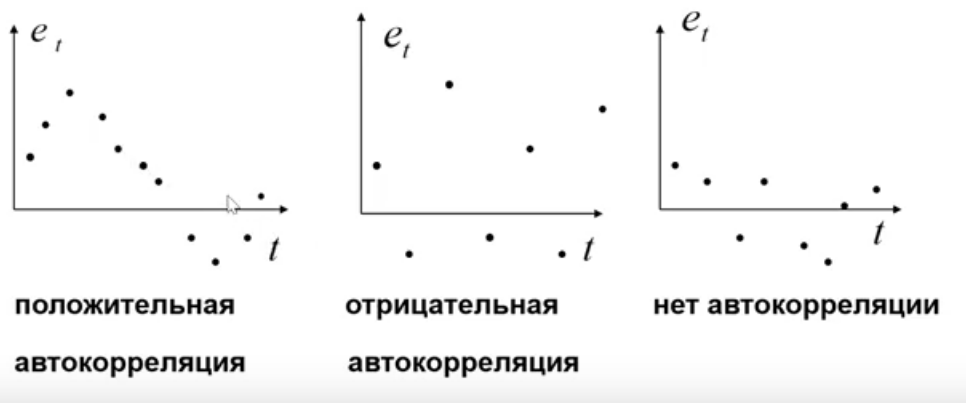
\includegraphics[scale = 0.5]{auto.png}

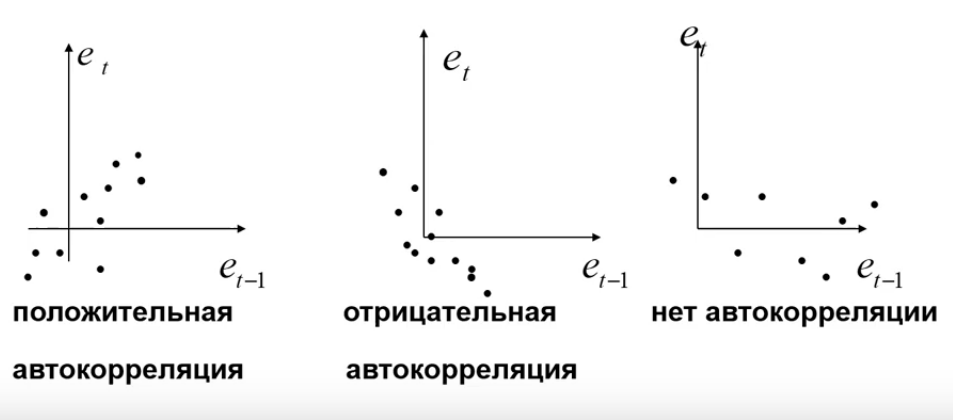
\includegraphics[scale = 0.5]{auto2.png}

\subsubsection{Тест серий}

Серия остатков - набор последовательных остатков одного знака

Если есть автокорреляция, то таких серий должно быть немного, но они достаточно длинные

\begin{center}
    \textit{Формальное описание}
\end{center}

\[\begin{cases}
    H_{0}: \rho = 0
    H_{1}: \textrm{ Имеет место автокорреляция первого порядка}
\end{cases}\]

\begin{enumerate}
    \item Оцениваются параметры уравнения регрессии
    \item Отмечаем знаки остатков
    \item \begin{enumerate}
        \item n - число всех наблюдений
        \item $N_{1}$ - число знаков +
        \item $N_{2}$ - число знаков - 
        \item K - число серий
    \end{enumerate}
    \item Если $K \leq K_{min}$, то имеет место положительная автокорреляция
    \item Если $K \geq K_{max}$, то имеет место отрицательная автокорреляция
    \item $k \sim N(\frac{2N_{1}N_{2}}{N_{1} + N_{2}} + 1; \frac{2N_{1}N_{2}(2N_{1}N_{2} - N_{1} - N_{2})}{(N_{1} + N_{2})^{2}(N_{1} + N_{2} - 1)})$
\end{enumerate}

\subsubsection{Статистика Дарбина-Уотсона}

\[d = \frac{\sum_{t = 2}^{T}(e_{t} - e_{t - 1})^{2}}{\sum_{t = 1}^{T}e_{t}^{2}}\]

\[\begin{cases}
    d \rightarrow 2 \Rightarrow \rho \approx 0 \\
    d \rightarrow 0 \Rightarrow \rho \approx 1 \\
    d \rightarrow 4 \Rightarrow \rho \approx -1 
\end{cases}\]

Надо проверять с учетом доверительных интервалов - статистики $d_{l}$ и $d_{u}$ мажорируют статистику d сверху независимо от параметров

Если d < $d_{l} \Rightarrow$ положительная автокорреляция

Если d > $d_{u} \Rightarrow$ нет положительной автокорреляции

Если между - неопределенность

\subsubsection{Устранение автокорреляции}

\begin{enumerate}
    \item Преобразовать исходные данные
    \item Использовать стандартные ошибки в форме Ньюи-Веста
    \item Использовать ММП
\end{enumerate}

Если мы знаем $\rho$ - можно произвести сдвиг 
\[Y_{t} - \rho Y_{t - 1} = \beta_{0}(1 - \rho) + \beta_{1}(X_{t} - \rho X_{t - 1}) + u_{t}, u_{t} - \textrm{некоррелированные ошибки}\]
\[Y^{*} = \beta_{0} + \beta_{1}X_{t}^{*} + u_{t}\]

$u_{t}$ удовлетворяют ТГМ

Теряется первое наблюдение

\textbf{Поправка Прайса-Уинстона}

Выражается из обобщенного метода МНК

\[Y^{*}_{1} = \sqrt{1 - \rho^{2}}Y_{1}\]

\[Y^{*}_{t} = Y_{t} - \rho Y_{t - 1}, t = 2, ..., T\]

\subsubsection{Оценка параметра автокорреляции}

\begin{enumerate}
    \item Выражение из Дарбина-Уотсона
    \item Процедура Кокрена-Уоркута
    \begin{enumerate}
        \item Оцениваем уравнение регресии и находим остатки
        \item Оцениваем регрессию остатков на предыдущие, получаем $\rho_{1}$
        \item Преобразуем исходные данные
        \item Повторяем 1 и 2, получаем $\rho_{2}$ 
        \item $|\rho_{1} - \rho_{2}| < \varepsilon \rightarrow \rho = \rho_{2}$
        \item Если процедура не сходится - могли не угадать порядок автокорреляции
    \end{enumerate}
    \item Двухшаговая процедура Дарбина
    \begin{enumerate}
        \item \[Y_{t} = \rho Y_{t - 1} + \beta_{0}(1 - \rho) + ...\]
        \item Оцениваем $\rho$
    \end{enumerate}
    \item Метод поиска Хилдрет-Лю на сетке
    \begin{enumerate}
        \item Подбираем $\rho$ для которого RSS минимальна
    \end{enumerate}
    \item Среди регрессоров встречается стохастический $Y_{t - 1}$
    \begin{enumerate}
        \item $\varepsilon$ удовлетворяют Марковской схеме 1-го уровня
        \item Тогда статистика Дарбина-Уотсона не применима из-за возникновения проблемы эндогенности
        \item \textbf{Используется h-статистика Дарбина}
        \item \[\begin{cases}
            H_0: \rho = 0 \\
            H_1: \rho \neq 0
        \end{cases}\]
        \item \(h = \hat \rho \sqrt{\frac{n}{1 - ns^{2}_{b_{Y(-1)}}}}\)
    \end{enumerate}
    \item Тест Бройша-Годфри
    \begin{enumerate}
        \item $H_0: $ нет автокорреляции возмущений
        \item $H_1: $ имеет место автокорреляция порядка p
        \item \[\begin{cases}
            H_0: \rho_1 = \rho_2 = \ldots = \rho_p = 0 \\
            H_1: \rho^{2}_{1} + \rho^{2}_{2} + \ldots + \rho^{2}_{P} \neq 0
        \end{cases}\]
        \item Проверяется гипотеза о том, что ошибки являются белым шумом
        \item \textit{Алгоритм}
        \begin{enumerate}
            \item Оцениваются параметры регрессии
            \[Y_t = \beta_{0} + \beta_{1}X_{t} + \varepsilon_t\]
            \item Сохраняются остатки регрессии
            \item Оцениваются параметры регрессии
            \[e_t = \beta_0 + \beta_1 X_t + r_1 e_{t - 1} + \ldots r_{P}e_{t - P} + \varepsilon_{t}\]
            \item Сохраняется $R^2$
            \item Тестовая статистика \[\chi^{2} = TR^{2}\]
            \item Если $\chi^{2} > \chi^{2}_{cr}$, то гипотеза отвергается
        \end{enumerate}
    \end{enumerate}
    \item \underline{Стандартные ошибки в форме Ньюи-Веста}
    \[var[\varepsilon] \sim \Omega = (w_{ij}), w_{ij} = 0, |i - j| > L\]
    \[\hat{var}[\hat{\beta}] = n(X'X)^{-1}\frac{1}{T}(\sum_{s = 1}^{T}e_{s}^{2}x_{s}x_{s}' + \sum_{j = 1}^{L} \sum_{t = j + 1}^{T} w_{j}e_{t}e_{t - j}(x_t x_{t - j}' + x_{t - j}x'_{t}))(X'X)^{-1}\]
    \item \underline{Q-статистика для проверки белошумности остатков}
    \begin{enumerate}
        \item Модель ARMA(p, q)
        \item \[
            \begin{cases}
                    H_0: \rho_1 = \ldots = \rho_m = 0 \\
                    H_1: \rho_1^2 + \ldots + \rho^2_m > 0
            \end{cases}
        \]
        \item \[
            Q_m = T\sum_{k = 1}^m r_k^2
        \]
        \item $r_k$ - выборочный коэффициент корреляции остатков $\varepsilon_t$ и $\varepsilon_{t - k}$
        \item m - гиперпараметр
        \item \[
            Q \sim \chi^{2}(m - p - q)
        \]
        \item Статистика Q используется и для проверки белошумности исходного ряда, тогда тестовая статистика имеет распределение $\chi^{2}(m)$
    \end{enumerate}
    \item \underline{Статистика Бокса-Льюнга} (для малых выборок)
    \begin{enumerate}
        \item \[Q_k = T(T + 2)\sum_{k = 1}^m \frac{1}{T - k}r_{k}^2\]
    \end{enumerate}
    \item \textit{Статистики хорошо работают, когда справа стоят экзогенные факторы, для временных рядов достаточно слабы}
\end{enumerate}

\subsection{Моделирование сезонности во временных рядах}

\subsubsection{Модели ARIMA с сезонностью}

\begin{enumerate}
    \item Включение набора дамми-переменных для каждого месяца кроме одного, чтобы избежать dummy trap
    \item Использование Y(-12)
\end{enumerate}

\subsubsection{SARIMA}

\begin{enumerate}
    \item Мультипликативная
    \begin{enumerate}
        \item \[(1 - \rho_1 L)\{\Delta ln(wpi_t) - \beta_0\} = (1 + \theta_1 L)(1 + \theta_{4, 1} L^4)\varepsilon_t\]
        
        \[\Delta ln(wpi_t) = \beta_0 + \rho_1\{\Delta ln(wpi_{t - 1}) - \beta_0\} + \theta_1 \varepsilon_{t - 1} + \theta_{4, 1} \varepsilon_{t - 4} + \theta_1 \theta_{4, 1} \varepsilon_{t - 5} + \varepsilon_t\]
        \item В общем виде SARIMA $(p, d , q) \times (P, D, Q)_s$:
        \[\rho(L^p) \rho_s(L^P) \Delta^d \Delta_s^D z_t = \theta(L^q) \theta_s(L^Q)\varepsilon_t\]
        \[\rho_s(L^P) = (1 - \rho_{s, 1}L^s - \rho_{s, 2}L^{2s} - ... \rho_{s, P}L^{Ps})\]
        \[\theta_s(L^Q) = (1 - \theta_{s, 1}L^s - \theta_{s, 2}L^{2s} - ... \theta_{s, P}L^{Qs})\]
        \item Можно подбирать параметры P и Q (сезонные лаги), а не только p и q $\rightarrow$ AIC, BIC
        \item Оценивается с помощью ММП
    \end{enumerate}
    \item Аддитивная
    \begin{enumerate}
        \item \[\Delta ln(wpi_t) = \beta_0 + \rho_1\{\Delta ln(wpi_{t - 1}) - \beta_0\} + \theta_1 \varepsilon_{t - 1} + \theta_4 \varepsilon_{t - 4} + \varepsilon_t\]
        
        \[(1 - \rho_1 L)\{\Delta ln(wpi_t) - \beta_0\} = (1 + \theta_1 L + \theta_4 L^4)\varepsilon_t\]
        \item Выше модель для квартальных данных (Добавляется четвертый лаг)
    \end{enumerate}
    \item В уравнение модели добавляются сезоннные лаги
\end{enumerate}

\subsubsection{Процедуры сглаживания ряда}

\begin{enumerate}
    \item STL Decomposition
    \item Экспоненциальное сглаживание
    \begin{enumerate}
        \item \[\hat Y_{t+1 | t} = \alpha Y_t + (1 - \alpha) \hat Y_{t|t - 1}\]
        \item ETS
        \[b_{t} = b_{t-1} + \beta u_t\]
        \[s_t = s_{t - 12} + \gamma u_t\]
        \[l_t = \ell_{t - 1} + b_{t - 1} + \alpha u_{t}\]
        \[y_t = \ell_{t - 1} + b_{t - 1} + s_{t - 12} + u_t\]
    \end{enumerate}
\end{enumerate}
\end{document}